
\chapter{Сплинты корневых систем и функции ветвления}
\label{cha:splints}


Сплинт корневой системы простой алгебры Ли возникает при изучении регулярных вложений редуктивных подалгебр. Сплинт можно использовать для получения правил ветвления. Мы показываем, что использование свойств сплинта в сочетании с разложением сингулярного элемента позволяет сильно упростить вычисление коэффициентов ветвления. 

Вложение  $\phi$ корневой системы $\Delta_1$ в корневую систему $\Delta$ -- это биективное отображение корней из $\Delta_{1}$ в (собственное) подмножество $\Delta$, коммутирующее с законом сложения векторов в $\Delta_{1}$ и $\Delta$.

\begin{equation*}
\phi:\Delta_1 \longrightarrow \Delta
\end{equation*}
\begin{equation*}
\phi \circ (\alpha + \beta) =\phi \circ \alpha + \phi \circ \beta,
\,\,\, \alpha,\beta \in \Delta_1
\end{equation*}

Заметим, что образ  $Im(\phi)$ не обязан обладать свойствами корневой системы за исключением правил сложения, эквивалентных правилам сложения в  $\Delta_{1}$ (для прообразов). Два вложения  $\phi_1$ и $\phi_2$  {\it расщепляют} корневую систему  $\Delta$ если она может быть представлена, как несвязное объединение образов $Im(\phi_1)$ и $Im(\phi_2)$.   
Термин {\it сплинт} (расщепление) предложил D. Richter в работе  \cite{richter2008splints}, где  были получены все сплинты для простых алгебр Ли. В работе так же упоминалось, что сплинт должен быть тесно связан с конструкцией веера вложения, определенной в главе \ref{cha:affine-lie-algebras} (См. Определение \ref{fan-definition}).

В данной главе мы изучаем связь между сплинтом и веером вложения для регулярных вложений редуктивных подалгебр ${\mathfrak a}$ в простую алгебру Ли $\gf$. Мы демонстрируем, что (при выполнении определенных условий, описанных в разделе \ref{sec:stems and multiplicity functions}) сплинт является естественным инструментом для изучения свойств редукции  $\gf$-модулей по отношению к подалгебре $\af\longrightarrow\gf$. Используя этот инструмент мы получаем основной результат данной главы -- однозначное соответствие между кратностями весов неприводимых модулей сплинта и коэффициентов ветвления для редуцированного модуля $L^{\mu}_{\gf\downarrow \af}$.

Затем мы обсуждаем аффинное расширение корневой системы допускающей сплинт и получаем новые соотношения, связывающие функции ветвления неприводимых модулей на модули конечномерных подалгебр (см. Раздел \ref{sec:splints-affine}).

\section{Вложения и сплинты}

\label{sec:Injections and splints}

Рассмотрим простую алгебру Ли $\gf$ и ее  регулярную подалгебру $\af \hookrightarrow \gf$, такую, что $\af$ -- редуктивную подалгебра $\af\subset \gf$ и корневые системы согласованы $\hf_{\af}^{\ast}\subset\hf_{\gf}^{\ast}$. Пусть $\af^{\mathfrak{s}}$ -- полупростое слагаемое в $\mathfrak{a}$, то есть  $\af=\af^{\mathfrak{s}} \oplus \uf(1)\oplus \uf(1)\oplus \dots$. Мы будем считать, что $\af^{\mathfrak{s}}$ -- собственная регулярная подалгебра и что $\af$ -- максимальная подалгебра с заданной  $\af^{\mathfrak{s}}$, то есть ранг $r$ подалгебры $\af$ равен рангу $\gf$.

Приведем два определения, введенные в работе \cite{richter2008splints}

\begin{definition}
Пусть $\Delta _{0}$ и $\Delta$ -- корневые системы с соответствующими весовыми решетками $P_{0}$ и $P$. Рассмотрим отображение
\begin{equation}
\phi :\left\{
\begin{array}{l}
\Delta _{0}\hookrightarrow \Delta , \\
P_{0}\hookrightarrow P.
\end{array}
\right.
\end{equation}
Оно называется ``вложением'', если \newline
\noindent (a) оно вкладывает $\Delta _{0}$ в $\Delta $, и \newline
\noindent (b) $\phi$ действует гомоморфно по отношению к группам сложения векторов в $P_{0}$ и $P$:
\[
\phi (\gamma )=\phi (\alpha )+\phi (\beta )
\]
для любой тройки $\alpha ,\beta ,\gamma \in P_{0}$, такой, что $\gamma =\alpha+\beta $.
\end{definition}

$\phi$ индуцирует вложение формальных алгебр: ${\mathcal{E}}_0\hookrightarrow \mathcal{E}$ и для образа ${\mathcal{E}}_i=\mathrm{Im}_{\phi}\left( {\mathcal{E}}_0\right)$ можно рассмотреть обратное отображение $\phi^{-1}:{\mathcal{E}}_i \longrightarrow {\mathcal{E}}_0$.

Заметим, что нужно различать два класса вложений: когда скалярное произведение (заданное формой Киллинга) в корневом пространстве $P_0$ инвариантно по отношению к  $\phi$ и когда оно не  $\phi$-инвариантно. Вложения первого класса называются ``метрическими'', второго -- ``неметрическими''. 

\begin{definition}
Корневая система $\Delta$ ``расщепляется'' на  $(\Delta _{1},\Delta _{2})$, если существует два вложения  $\phi _{1}:\Delta _{1}\hookrightarrow \Delta $ и $\phi _{2}:\Delta _{2}\hookrightarrow \Delta $, где (a) $\Delta $ -- несвязное объединение образов $\phi _{1}$ и $\phi _{2}$, и (b) ни ранг  $\Delta _{1}$, ни ранг  $\Delta _{2}$ не превосходит ранга $\Delta $.
\end{definition}

Эквивалентно, можно сказать, что  $(\Delta_1,\Delta_2)$  -- ``сплинт'' (расщепление)  $\Delta$ и мы можем обозначить его через $\Delta \approx (\Delta_1,\Delta_2)$. Каждая из компонент  $\Delta_1$ и $\Delta_2$ называется ``стеблем'' сплинта $(\Delta_1,\Delta_2)$.

Чтобы показать связь веера вложения со сплинтом рассмотрим случай, когда один из стеблей $\Delta _{1}=\Delta _{\af}$  является подсистемой корневой системы. 

Сплинт $\Delta \approx (\Delta _{1},\Delta _{2})$ называется ``инъективным'', если $\Delta _{1}=\Delta _{\af}$, -- подсистема корневой системы $\Delta $, соответствующая регулярной редуктивной подалгебре $\af\hookrightarrow \gf$. 

В случае инъективного сплинта второй стебель $\Delta _{\sfr}:=\Delta_{2}=\Delta \setminus \Delta _{\af}$ может быть переписан как произведение (аналогично формуле (\ref{eq:142})) и определяет веер вложения  $\Gamma _{\af\hookrightarrow \gf}$. Обозначим через $\Delta_{\mathfrak{s}0}$ кообраз второго вложения $\phi:\Delta_{\mathfrak{s}0}\to \Delta_{\gf}$. Верна следующая гипотеза.

\begin{conjecture}
Каждый инъективный сплинт $\Delta \approx (\Delta _{\af},\Delta _{\sfr})$ определяет веер вложения с носителем $\left\{ \xi \right\} _{\af\rightarrow \gf}$, задающимся произведением
\begin{equation}
\prod_{\beta \in \Delta _{\sfr}^{+}}\left( 1-e^{-\beta }\right)
=-\sum_{\gamma \in P}s(\gamma )e^{-\gamma }\quad   \label{splint product}
\end{equation}
\end{conjecture}

В случае инъективного сплинта мы можем сказать, что подалгебра $\af\hookrightarrow \gf$ расщепляется $\Delta$ (и назовем $\af$ ``расщепляющей подалгеброй'' алгебры $\gf$).  Сплинты были классифицированы в работе \cite{richter2008splints}  и первые три класса сплинтов в этой классификации инъективны. 

\section{Как стебли определяют функции кратности}

\label{sec:stems and multiplicity functions}

В этом разделе мы рассмотрим свойства инъективных сплинтов $\Delta \approx (\Delta _{\af},\Delta _{\sfr})$. Мы покажем, что в этом случае вычисление коэффициентов ветвления для расщепляющего вложения $\af\hookrightarrow\gf$ эквивалентно нахождению кратностей весов неприводимого $\sfr$-модуля $L_{\sfr}^{\nu }$ с определенным старшим весом $\nu $. Заметим, что алгебра $\sfr$ не обязательно должна быть подалгеброй $\gf$.

Вернемся к соотношению (\ref{eq:124}). В данном случае операция проекции тривиальна, поэтому после умножения обеих сторон на  $R_{\af}$ получаем:
\begin{equation}
\frac{1}{\prod_{\beta \in \Delta _{\sfr}^{+}}(1-e^{-\beta })}\Psi _{\gf}^{\left( \mu \right) }=\sum_{\nu \in P_{\af}^{+}}b_{\nu}^{(\mu )}\Psi _{\af}^{\left( \nu \right) }.
\label{singular main-2}
\end{equation}
Здесь первый множитель в левой части -- это формальный элемент, обратный к вееру $\Gamma _{\af\rightarrow \gf}$. Рассмотрим модуль старшего веса $L_{\sfr}^{\nu }$. Вложение $\phi :\Delta _{\sfr\,0}\longrightarrow \Delta_{\gf}$ переводит сингулярный элемент  $\Psi _{\sfr}^{\left( \nu\right) }$ в $\Psi _{\gf}^{\left( \mu \right) }$. Применяя обратный морфизм $\phi ^{-1}$ к произведению $\left( \prod_{\beta \in \Delta_{\sfr}^{+}}(1-e^{-\beta })\right) ^{-1}\phi \left( \Psi _{\sfr}^{\left( \nu \right) }\right) $, мы получаем характер модуля $L_{\sfr}^{\nu }$,

\begin{equation}
\phi ^{-1}\left( \frac{1}{\prod_{\beta \in \Delta _{\sfr%
}^{+}}(1-e^{-\beta })}\phi \left( \Psi _{\sfr}^{\left( \nu \right)
}\right) \right) =\frac{1}{\prod_{\beta \in \Delta _{\sfr0
}^{+}}(1-e^{-\beta })}\Psi _{\sfr}^{\left( \nu \right) }=\mathrm{ch}%
\left( L_{\sfr}^{\nu }\right) .  \label{inverse for stem}
\end{equation}
Наша задача состоит в том, чтобы доказать, что сингулярный элемент $\Psi _{\gf}^{\left(\mu\right) }$ содержит элемент $\Psi _{\sfr}^{\left( \xi \right) }$ для модуля $L_{\sfr}^{\xi }$, однозначно определяемого модулем $L_{\gf}^{\mu }$ и что коэффициенты ветвления $b_{\nu }^{(\mu )}$ в правой части равенства (\ref{singular main-2}) совпадают с кратностями $m_{\zeta }^{\left( \xi\right) }$ соответствующих весов в $\mathcal{N}_{\sfr}^{\xi }$ .

Для неприводимого модуля старшего веса $L_{\gf}^{\mu }$ сингулярный элемент $\Psi _{\gf}^{\left( \mu \right) }$ -- это элемент $\mathcal{E}$, соответствующий сдвинутой орбите группы Вейля веса $\left( \mu +\rho\right) \in P^{+}$, со знаковой функцией $\epsilon \left( w\right) $. Удобно использовать также не сдвинутые сингулярные элементы
\begin{equation}
\Phi ^{\left( \mu \right) }:=\Psi ^{\left( \mu \right) }e^{\rho }.
\label{definition Phi}
\end{equation}
В этих обозначениях соотношение (\ref{singular main-2}) имеет вид
\begin{equation}
\frac{e^{\rho _{\gf}-\rho _{\af}}}{\prod_{\beta \in \Delta _{\frak{%
s}}^{+}}(1-e^{-\beta })}\Phi _{\gf}^{\left( \mu \right) }=\sum_{\nu \in
P_{\af}^{+}}b_{\nu }^{(\mu )}\Phi _{\af}^{\left( \nu \right) }.
\label{singular main-3}
\end{equation}
Орбита, связанная с  $\Phi _{\gf}^{\left( \mu \right) }$, полностью определяется набором ребер $\left\{ \lambda _{i}\right\} _{i=1,\dots ,r}$ построенным из конца вектора старшего веса $\mu +\rho $. Для $\mu=\sum m_{i}\omega _{i}$ эти ребра равны
\begin{equation}
\lambda _{i}=-\left( m_{i}+1\right) \alpha _{i},\quad i=1,\dots ,r.
\label{edge}
\end{equation}
Каждая формальная экспонента $e^{\mu +\rho +\lambda _{i}}$ in $\Phi _{\gf}^{\left( \mu \right) }$ снабжена знаковым коэффициентом  $\epsilon =(-)$. Можно определить $\Phi_{\gf}^{\left( \mu \right) }$ следующим свойством. Рассмотрим любую пару ребер $\lambda _{i},\lambda _{j}$ и соответствующие веса $\mu +\rho $, $\mu +\rho +\lambda _{i}$ и $\mu +\rho +\lambda _{j}$. 
Применим отражение $s_{\alpha _{i}}$ (или $s_{\alpha _{j}}$),
\begin{equation}
s_{\alpha _{i}}\circ \left\{
\begin{array}{l}
\left( \mu +\rho \right)  \\
\left( \mu +\rho +\lambda _{i}\right)  \\
\left( \mu +\rho +\lambda _{j}\right)
\end{array}
\right. =\left\{
\begin{array}{l}
\left( \mu +\rho +\lambda _{i}\right)  \\
\left( \mu +\rho \right)  \\
\left( \mu +\rho +\lambda _{i}-(m_{j}+1)s_{\alpha _{i}}\circ \alpha
_{j}\right)
\end{array}
\right.   \label{reflected triple}
\end{equation}

\begin{Prop}
Ребро  $\lambda _{i,j}$ сингулярного элемента $\Phi _{\gf}^{\left( \mu \right) }$, начинающееся в весе $\left( \mu +\rho +\lambda _{i}\right) $ и направленное вдоль корня $-s_{\alpha _{i}}\circ \alpha _{j}$ имеет такую же длину, выраженную в длинах корня $(s_{\alpha_{i}}\circ \alpha _{j})$, как и $\lambda _{j}$ в длинах $\alpha _{j}$. (Это же верно для ребра $\lambda _{j,i}$, его длина в единицах $(s_{\alpha _{j}}\circ\alpha _{i})$ равна длине $\lambda _{i}$ в единицах $\alpha _{i}$.)
\label{diagram property}
\end{Prop}

В $\Phi _{\gf}^{\left( \mu \right) }$ элементы $e^{\left( \mu+\rho +\lambda_{i}-(m_{j}+1)s_{\alpha _{i}}\circ \alpha _{j}\right) }$ и $e^{\left( \mu +\rho +\lambda _{j}-(m_{i}+1)s_{\alpha_{j}}\circ \alpha_{i}\right) }$ имеют знаковый коэффициент  $\epsilon =(+)$.

Вспомним, что только три типа сплинтов инъективны и имеют естественную связь с ветвлениями. Ниже мы приводим часть таблицы сплинтов из работы \cite{richter2008splints}, соответствующую инъективным сплинтам:
\begin{equation}
  \label{eq:128}
  \begin{array}{cc||c|c}
    \hbox{тип} & \hspace{0.25in}\Delta \hspace{0.25in} & \hspace{0.25in}\Delta
    _{\af}\hspace{0.25in} & \hspace{0.25in}\Delta _{\sfr}\hspace{0.25in}
    \\ \hline\hline
    \hbox{(i)} & G_{2} & A_{2} & A_{2} \\
    & F_{4} & D_{4} & D_{4} \\ \hline
    \hbox{(ii)} & B_{r}(r\geq 2) & D_{r} & \oplus ^{r}A_{1} \\
    (*)& C_{r}(r\geq 3) & D_{r} & \oplus ^{r}A_{1} \\ \hline
    \hbox{(iii)} & A_{r}(r\geq 2) & A_{r-1}\oplus u\left( 1\right)  & \oplus
    ^{r}A_{1} \\
    & B_{2} & A_{1}\oplus u\left( 1\right)  & A_{2}
  \end{array}
\end{equation}


Каждая строка в таблице соответствует сплинту  $(\Delta _{\af},\Delta _{\sfr})$  корневой системы $\Delta $. В случае первых двух типов и  $\Delta _{\af}$, и $\Delta _{\sfr}$ вложены метрически. Стебли для первого типа эквивалентны, а для второго -- нет. В случае третьего типа сплинтов только корневая система $\Delta _{\af}$ вложена метрически. Слагаемые $u\left( 1\right) $ добавлены, чтобы совпадали ранги $r_{\af}=r$. Такая добавка не меняет основных свойств ветвления, но позволяет использовать кратности весов $\sfr$-модулей без последующей проекции весов.

Второй инъективный сплинт типа (ii), отмеченный звездочкой в таблице (\ref{eq:128}), не порождает дополнительного $\sfr$-модуля и ветвление в этом случае связано со сплинтом более сложным образом. Мы не рассматриваем здесь этот случай.

Сплинт индуцирует разложение множества $S=S_{\frak{c}}\cup S_{\frak{d}}$, где $S_{\frak{c}}=S\cap S_{\af}$ и $S_{\frak{d}}=S\cap S_{\sfr}$.  Легко проверить, что для любого инъективного сплинта подмножество  $S_{\frak{d}}$ не пусто. Следовательно, в множестве $\left\{ \lambda
_{i}\right\} _{i=1,\dots ,r}$ всегда найдется простые корни $\beta_{k}\in \Delta _{\sfr}$ и орбита, соответствующая $\Phi _{\gf}^{\left( \mu \right) }$ будет содержать ребра
\begin{equation}
\lambda _{k}=-\left( m_{k}+1\right) \beta _{k}  \label{beta edge},
\end{equation}
построенные из веса  $\mu +\rho $.  Так как $\Delta _{\af}$ -- корневая система и для любой пары простых корней из $S_{\frak{c}}$ выполнено свойство \ref{diagram property}, элемент  $\Phi _{\gf}^{\left( \mu \right) }$ является сингулярным элементом для набора  $\af$-модулей. Рассмотрим корень $\beta _{l}\in \Delta _{\sfr}$, кообраз которого в  $\Delta _{\sfr0}$  простой. В разделе \ref{sec:appendix} мы показываем, что для каждого такого $\beta _{l}$ существует корень  $\alpha _{l}\in S_{\frak{c}}$, такой, что $\beta _{l}=\alpha _{l}+\beta _{k}$. Легко видеть, что в этом случае соответствующее ребро пересекает гиперплоскость, ограничивающую главную камеру Вейля $\bar{C_{\af}}$ и ортогональную к корню $\alpha _{l}$,
\begin{equation}
s_{\alpha _{l}}\left( \mu +\rho -p\beta _{l}\right) =s_{\alpha _{l}}\left(
\mu +\rho \right) -ps_{\alpha _{l}}\beta _{l}=\mu +\rho -p\beta _{l},
\label{intersection}
\end{equation}
\begin{equation}
\mu +\rho -s_{\alpha _{l}}\left( \mu +\rho \right) =\left( m_{l}+1\right)
\alpha _{l}=\left( m_{l}+1\right) \beta _{l}-\left( m_{l}+1\right) \beta
_{k}=p\beta _{l}-ps_{\alpha _{l}}\beta _{l}.  
\label{intersection-2}
\end{equation}
Следовательно,  $p=\left( m_{l}+1\right) $ и  $s_{\alpha _{l}}\beta_{l}=\beta _{k}$. Теперь применим оператор $s_{\beta _{k}}$ и заметим, что ребро, построенное вдоль корня $s_{\beta _{k}}\alpha _{l}$ из веса $s_{\beta _{k}}(\mu +\rho )$ тоже равно $-ps_{\beta _{k}}\alpha _{l}$. Значит, для тройки корней  $\beta _{k},\beta _{l}$ и $s_{\beta _{k}}\alpha _{l}$ in $\Delta _{\sfr}$ ребра $\lambda_{k}=-\left( m_{k}+1\right) \beta _{k}$, $\lambda _{l}=-\left(m_{l}+1\right) \beta _{l}$ и $\lambda _{kl}=-\left( m_{l}+1\right)s_{\beta _{k}}\alpha _{l}$ удовлетворяют свойству \ref{diagram property}.
Эту процедуру можно продолжить далее в двумерном подпространстве, заданном корнями $\beta _{k}$ и $\beta _{l}$ и показать, что множество формальных экспонент, снабженных соответствующими знаковыми множителями, составляет кообраз сингулярного элемента модуля подалгебры в  $\frak{
s}$ (ранг этой подалгебры $r=2$).

Аналогичное рассуждение  можно провести для любого положительного корня $\beta _{l}\in \Delta $, являющегося простым в $\Delta _{\sfr0}$ и, соответственно, для любой подалгебры ранга $r=2$ в $\sfr$. То есть чтобы ``найти'' сингулярный элемент $\sfr$-модуля в $\Phi_{\gf}^{\left( \mu \right) }$ необходимо сгруппировать с ним дополнительные формальные элементы  $\left\{ -e^{\mu +\rho-\left( m_{l}+1\right) \beta _{l}}|\beta _{l}\in S_{\frak{c}}\right\}.$ Эта процедура определяет начальные ребра диаграммы $\phi ^{-1}\left( \Phi _{\sfr}^{\widetilde{\mu }}\right) $. Как следует из процедуры восстановления, старший вес $\widetilde{\mu }$ полностью определяется весом $\mu $, эти веса имеют следующие индексы Дынкина:
\begin{equation}
\mu =\sum m_{k}\omega _{k}\qquad \Longrightarrow \quad \widetilde{\mu }=\sum
m_{k}\widetilde{\omega }_{k} . \label{new h weight}
\end{equation}
Следующим шагом необходимо проверить, что образ $\phi\left(\Phi^{(\tilde \mu)}_{\sfr}\right)$ содержится в $\bar C_{\af}$ и множество $\phi\left(\Phi^{(\tilde\mu)}_{\sfr}\right)\setminus \left.\Phi^{(\mu)}_{\gf}\right|_{\bar C_{\af}}$ соответствует весам на границе $\bar C_{\af}$ (включая подмножество $\left\{-e^{\mu+\rho-(m_l+1)\beta_l}|\; \beta_l\in S_{\frak{c}}\right\}$). Предположим, что это условие выполнено и вернемся к соотношению (\ref{singular main-3}). Можно добавить к $\Phi _{\gf}^{\left( \mu \right) }$ пары формальных элементов, построенные выше, с противоположными знаками: $\epsilon \left( w\right)|_{w\in W_{\sfr}}$  и  $-\epsilon \left( w\right) |_{w\in W_{\sfr}}$. 
Припишем знаки $\epsilon \left( w\right) |_{w\in W_{\sfr}}$ элементам, веса которых попадут в главную камеру $\bar{C_{\af}}$. К соседним камерам $\bar{C}_{\af}^{(l)}$ относятся те же элементы, но  с противоположным знаком  (Эти камеры связаны с главной простыми отражениями $s_{\alpha _{l}}$, так что противоположные знаки $-\epsilon \left( w\right) |_{w\in W_{\sfr}}$ здесь естественны). Можно повторить эту процедуру и получить дополнительные сингулярные веса в любой камере Вейля $\bar{C_{\af}^{(m)}}$, причем эти веса будут иметь знаки, противоположные знакам в соседних камерах. То есть не меняя элемент $\Phi _{\gf}^{\left( \mu \right) }$ его можно представить в виде суммы
\begin{equation}
\Phi _{\gf}^{\left( \mu \right) }=\sum_{w\in W_{\af}}w\circ \left(
e^{\rho _{\af}}\Psi ^{\widetilde{\mu }+\rho _{\sfr}}\right)
\label{singular final}
\end{equation}
где вес $\widetilde{\mu }=\sum m_{k}\omega _{\sfr}^{k}$ был введен выше. Разложение (\ref{singular final}) позволяет применить множитель $\left( \prod_{\beta \in \Delta _{\sfr}^{+}}(1-e^{-\beta })\right) ^{-1}$ к каждому слагаемому сингулярного элемента  $\Phi _{\gf}^{\left( \mu \right)}$ по отдельности, так как множества весов различных слагаемых Вейля не пересекаются. Воспользовавшись изоморфизмом  $\phi $ мы видим, что в главной камере Вейля  $\bar{C_{\af}}$ множество весов, порожденное действием $\left( \prod_{\beta\in \Delta _{\sfr}^{+}}(1-e^{-\beta })\right)^{-1}$ изоморфно весовой диаграмме  $\mathcal{N}_{\sfr}^{\widetilde{\mu }}$  модуля  $L_{\sfr}^{\widetilde{\mu }}$ алгебры $\sfr$. Теперь можно ограничить равенство (\ref{singular main-3}) на главную камеру Вейля $\bar{C_{\af}}$ и получить основной результат этого раздела:
\begin{Prop}
\begin{equation}
\frac{e^{\rho _{\gf}}}{\prod_{\beta \in \Delta _{\sfr%
}^{+}}(1-e^{-\beta })}\left( \Psi ^{\widetilde{\mu }+\rho _{\sfr%
}}\right) =\sum_{\widetilde{\nu }\in \mathcal{N}_{\sfr}^{\widetilde{\mu }%
}}M_{\left( \sfr\right) \widetilde{\nu }}^{\widetilde{\mu }}e^{\left(
\mu -\phi \left( \widetilde{\mu }-\widetilde{\nu }\right) \right)
}=\sum_{\nu \in P_{\af}^{++}}b_{\nu }^{(\mu )}e^{\nu }.
\label{singular main-4}
\end{equation}
Любой вес с ненулевой кратностью, входящий в правую часть равенства, равен одному из старших весов в разложении. Кратность $M_{\left( \sfr
\right) \widetilde{\nu }}^{\widetilde{\mu }}$ веса  $\widetilde{\nu}\in \mathcal{N}_{\sfr}^{\widetilde{\mu }}$ определяет коэффициент ветвления  $b_{\nu }^{(\mu )}$ для старшего веса $\nu =\left( \mu-\phi \left( \widetilde{\mu }-\widetilde{\nu }\right) \right) $:
\[
b_{\left( \mu -\phi \left( \widetilde{\mu }-\widetilde{\nu }\right) \right)
}^{(\mu )}=M_{\left( \sfr\right) \widetilde{\nu }}^{\widetilde{\mu }}.
\]
\end{Prop}

\section{Примеры}
\label{sec:examples}
\begin{example}
\label{example-1}
Рассмотрим алгебру Ли $A_{2} =\bf{sl}(3)$ и ветвление ее неприводимого модуля $L^{[3,2]}_{A_{2}}$ по отношению к редуктивной подалгебре $A_{1}\oplus u(1)$. Корневая система  $\Delta _{\af}= \Delta_{A_{1}\oplus u(1)}$ содержит простой корень $\alpha_1=e_1-e_2$ алгебры $A_{2}$. Сингулярный элемент $\Psi^{[3,2]}_{\af}$ раскладывается в сумму образов сингулярных элементов  модулей алгебры $A_{1}\oplus A_{1}$. Коэффициенты ветвления $b_{\nu }^{[ 3,2 ] }$ совпадают с кратностями весов модуля $L^{[3,2]}_{A_{1}\oplus A_{1}}$ (см. Рисунок. \ref{fig:a2_splint}).

  \begin{figure}[h!bt]
  \noindent\centering{
   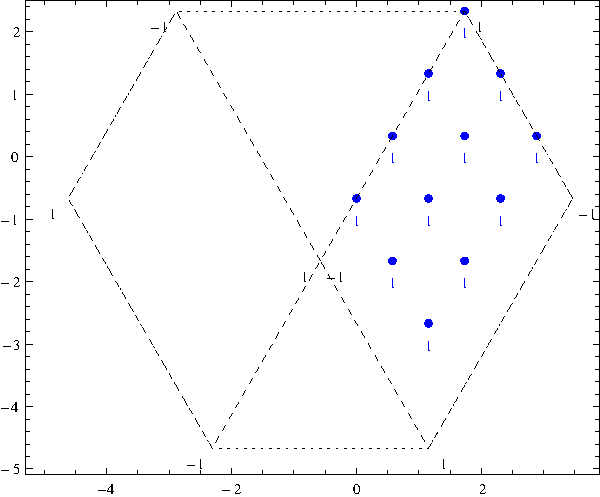
\includegraphics[width=80mm]{a2-a1}
  }
  \caption{Орбита группы Вейля (точечный контур), соответствующая сингулярному элементу $L^{[3,2]}_{A_{2}}$ и ее разложение в сумму образов сингулряных элементов модулей  $L^{[3,2]}_{A_{1}\oplus A_{1}}$ (пунктирные контуры). Кратности весов модуля $L^{[3,2]}_{A_{1}\oplus A_{1}}$ совпадают  с коэффициентами ветвления для редукции $L^{[3,2]}_{A_{2}\downarrow A_{1}\oplus u(1)}$.}

 \label{fig:a2_splint}
\end{figure}
\end{example}
\begin{example}
\label{example-2}
 Рассмотрим алгебру Ли $B_{2}= \bf{so}(5)$ и редукцию ее неприводимого модуля  $L^{[3,2]}$ на модули редуктивной подалгебры  $A_{1}\oplus u(1)$ с корневой системой, натянутой на первый простой корень $\alpha_1=e_1-e_2$ алгебры $B_{2}$. Сингулярный элемент $\Psi^{[3,2]}_{B_{2}}$ раскладывается в сумму образов сингулярных элементов модулей $A_{2}$ и коэффициенты ветвления совпадают с кратностями весов в модуле $A_{2}$ (см. Рисунок \ref{fig:b2_splint}).

  \begin{figure}[h!bt]
  \hspace*{-1.2cm}

   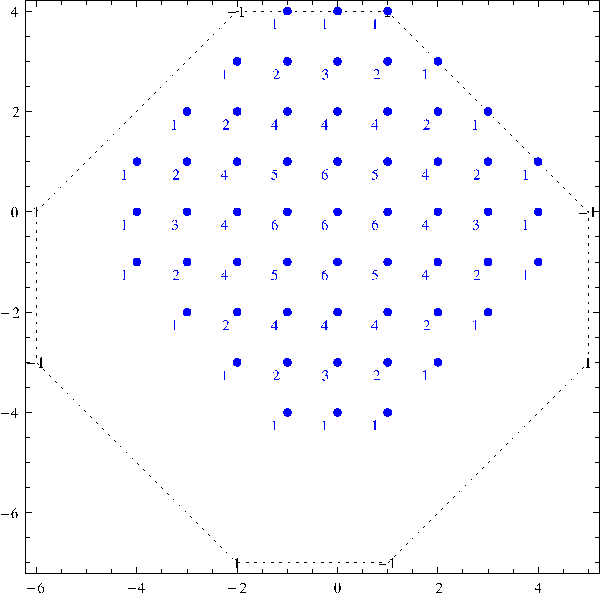
\includegraphics[width=65mm]{b2}
   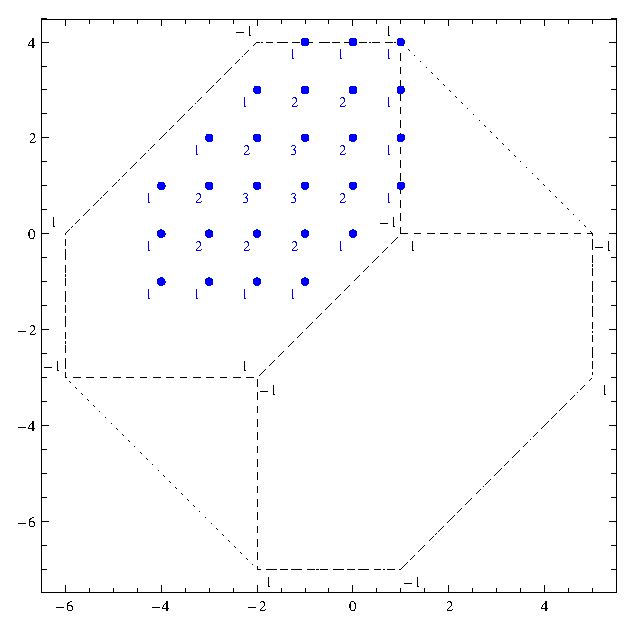
\includegraphics[width=65mm]{b2-a2-a1}
  \caption{Веса модуля  $L^{[3,2]}$ алгебры  $B_{2}$ показаны точками на левом рисунке (кратности подписаны). Контур сингулярного элемента показан коротким пунктиром. На правом рисунке представлено разложение сингулярного элемента $\Psi_{B_{2}}(L^{[3,2]}_{B_{2}})$ в сумму образов сингулярных элементов $\Psi_{A_{2}}(L^{[3,2]})$ (длинный пунктир). Кратности весов модуля $L^{[3,2]}_{A_{2}}$ совпадают с коэффициентами ветвления для редукции $L^{[3,2]}_{B_{2}\downarrow A_{1}\oplus u(1)}$.}

 \label{fig:b2_splint}
\end{figure}
\end{example}

\vspace{10mm}
\begin{example}
  Алгебра Ли  $G_{2}$ содержит регулярную подалгебры  $A_{2}$ с корневой системой $\Delta_{\af}=\Delta_{A_{2}}$, содержащей длинные корни $G_{2}$. Рассмотрим ветвление неприводимого модуля $L_{G_{2}}^{(3,2)}$ на модули подалгебры $A_{2}$. Сингулярный элемент $\Psi_{G_{2}}(L^{[3,2]})$ раскладывается в сумму образов сингулярных элементов  $\Psi_{A_{2}}(L^{[3,2]})$ и коэффициенты ветвления совпадают с кратностями весов модуля $L^{[3,2]}_{A_{2}}$ (см. Рисунок \ref{fig:g2_splint}).


  \begin{figure}[h!bt]
  \noindent\centering{
   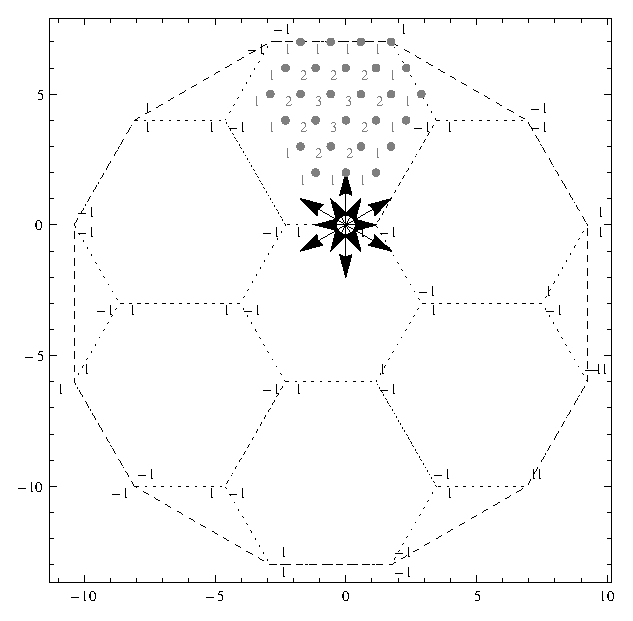
\includegraphics[width=120mm]{g2}
  }

  \caption{Орбита группы Вейля  (короткий пунктир) для сингулярного элемента  $\Psi_{G_{2}}(L^{[3,2]})$ и его разложение в сумму образов сингулярных элементов модулей алгебры $A_{2}$ (длинный пунктир). Кратности весов модуля $L^{[3,2]}_{A_{2}}$ совпадают с коэффициентами ветвления для редукции $L^{[3,2]}_{G_{2}\downarrow A_{2}}$.}


 \label{fig:g2_splint}
\end{figure}

\end{example}

\section{Сплинты классических алгебр Ли}
\label{sec:appendix}
%%%%%%%%%%%%%%%%%%%%%%%%%%%%%%%%%%%%%%%%%%%%%%%%%%%%%%%%%%%%%
Покажем, что для инъективного сплинта классической алгебры Ли выполняется следующее свойство:
\begin{Prop}
Пусть $\Delta \approx (\Delta _{\af},\Delta _{\sfr})$ -- инъективный сплинт с разложением множества простых корней  $S=S_{\frak{c}}\cup S_{\frak{d}}$, где $S_{\frak{c}}=S\cap S_{\af}$ и $S_{\frak{d}}=S\cap S_{\sfr}$.

Тогда для каждого простого корня  $\beta \in S_{\sfr}$ существует пара корней  ( $\alpha $ ,$\beta ^{\prime }$), где $\alpha \in $ $S_{\frak{c}},\beta ^{\prime }\in S_{\sfr}$, такая, что $\alpha =\beta-\beta ^{\prime }$
\end{Prop}
\begin{itemize}
\item
Тип 1. $\Delta _{G_{2}}\approx (\Delta _{A_{2}},\Delta
_{A_{2}}).$

 \begin{figure}[h!bt]
  \noindent\centering{
   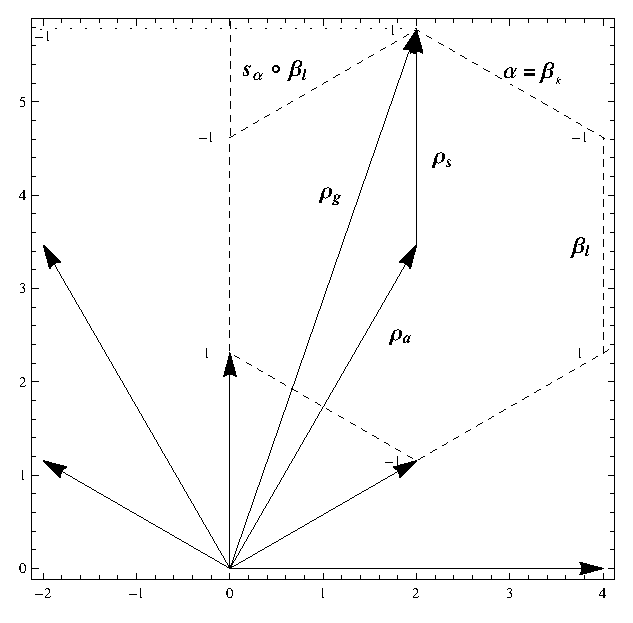
\includegraphics[width=100mm]{g2-roots}
  }
  \caption{Положительные корни $G_{2}$ и образование сингулярного элемента $\Phi^{(0)}_{\mathfrak{s}}$ в главной камере Вейля алгебры $\af=A_{2}$.}
  \label{fig:g2-roots}
\end{figure}
Здесь оба стебля метрические и соответствующие корневые системы эквивалентны. На Рисунке \ref{fig:g2-roots} показана часть сингулярного элемента $\Phi_{G_{2}}^{\left( 0\right) }$. Границы  $\bar{C_{\frak{a}}}$ изображены пунктирными линиями, начинающимися в центре сингулярного элемента. Они содержат ребро $\lambda _{2}=-\alpha _{2}=-\beta _{2}$ и корни $-\beta _{1}=-s_{\alpha _{2}}\circ \beta _{3}$ и $ -\beta _{3}$
($\beta _{3}$ показан, как $\beta _{l}$). Для корня $\beta_{1}$ искомая пара -- это  $(\alpha _{1}, \beta _{2})$: $\alpha _{1}=\beta _{1}-\beta _{2}$. Ребро $\lambda _{2,3}^{\sfr}=\beta _{3}$ равно  $\lambda _{1}^{\frak{s}}=\beta _{1}=s_{\alpha _{2}}\circ \beta _{3}$ и  $\sfr$-модуль получает индекс Дынкина $m_{1}$  и наследует второй индекс $m_{2}$. В этом частном случае  $m_{1}=m_{2}=0$.  Общий случай с начальным модулем $L^{\mu }$, где $\mu =m_{1}\omega _{1}+m_{2}\omega _{2}$, может быть рассмотрен аналогично: необходимо найти ребро $\lambda _{2}=-\left(
m_{2}+1\right) \beta _{2}$ и положить $\lambda_{1}^{\sfr}=-\left( m_{1}+1\right) \beta _{1}$, его конец принадлежит границе $\bar{C_{\af}}$. Отражение $s_{\beta_{2}} $ переводит $\beta _{1}$ в $\beta _{3}$ и соответствующее ребро
$\lambda _{2,3}^{\sfr}=-\left( m_{1}+1\right) \beta _{3}$ имеет длину $\left( m_{1}+1\right) $. Теперь рассмотрим ребра $\lambda _{1}^{\sfr}$ (или $\lambda _{2,3}^{\sfr} $) и $\lambda _{1,3}^{\sfr}$ (или $\lambda _{2,3,1}^{\sfr}$), и обнаружим, что они принадлежат границе  $\bar{C_{\af}}$ и Вейлевская симметрия предсказывает, что $\lambda _{1,3}^{\sfr}=-\left( m_{2}+1\right)\beta _{3}$ ($\lambda _{2,3,1}^{\sfr}=-\left( m_{2}+1\right) \beta _{1}$) . Наконец, ребро $\lambda _{1,3,2}^{\sfr}=-\left(m_{1}+1\right) \beta _{2}$ замыкает многогранник. Его вершины соответствуют весам сингулярного элемента $\Phi _{\sfr}^{\left( \widetilde{\mu }\right) }=\sum_{w\in W_{\sfr}}\varepsilon \left( w\right) e^{w\circ \left(
\widetilde{\mu }+\rho_{\sfr}\right) }$ модуля $L_{\sfr}^{\left( \widetilde{\mu }\right) }$, где $\widetilde{\mu }=m_{1}\widetilde{\omega }_{1}+m_{2}\widetilde{\omega }_{2}$. Заметим, что в этом случае знаковые множители можно получить прямо в первоначальной весовой системе, так как стебли метрические.
\item
Тип 1. $\Delta _{F_{4}}\approx (\Delta _{D_{4}},\Delta_{D_{4}}).$

Оба стебля здесь метрические и соответствующие корневые системы эквивалентны.  Система $\Delta _{D_{4}}$ подалгебры $\frak{a=}D_{4}$ формируется множеством $\left\{ \pm e_{i}\pm e_{j}\right\} _{|i,j=1,\ldots 4,\; i\neq j}.$ Простые корни $S_{\frak{c}}$ -- это $\left\{e_{2}-e_{3},e_{3}-e_{4}\right\} $ и $S_{\frak{d}}=\left\{ e_{4},\frac{1}{2}\left(e_{1}-e_{2}-e_{3}-e_{4}\right) \right\} $.
Для модуля $L^{\mu }$, где $\mu =\sum m_{k}\omega _{k}$ рассмотрим ребро $\lambda _{3}=-\left( m_{3}+1\right) e_{4}=-\left( m_{3}+1\right)
\beta _{3}$.
Построим ребро $\lambda _{2}^{\sfr}=-\left( \widetilde{m}_{2}+1\right) \beta _{2}$. Искомая пара корней -- это $\left(\alpha_{2}=e_{3}-e_{4},\beta _{3}\right) $. Пересечение  $\lambda _{2}^{\sfr}$ с  $\alpha _{2}$-границей камеры $\bar{C_{\af}}$ определяет длину $\lambda _{2}^{\sfr}=-\left( m_{2}+1\right) \beta _{2}$ и длины ребра $\lambda _{3,2}^{\sfr}$ равна длине $\lambda _{2}^{\sfr}$. Далее рассмотрим ребро $\lambda _{2}^{\sfr}=-\left( m_{2}+1\right) \beta _{2}$ и пару $\left( \alpha_{1}=e_{2}-e_{3},\beta _{1}=e_{2}\right) $. Длина   $\lambda _{1}^{\sfr}$ становится равной $\lambda_{1}^{\sfr}=-\left( m_{1}+1\right) \beta _{1}$. Продолжаем эту процедуру, пока не замкнем многогранник. Ребра, направленные вдоль корней типа $\alpha_4$, $\alpha _{4}=\beta_{4}=$ $\frac{1}{2}\left( e_{1}-e_{2}-e_{3}-e_{4}\right) $, рассматриваются аналогично и, наконец, сингулярный элемент $\Phi_{\sfr}^{\left( \widetilde{\mu }\right) }=\sum_{w\in W_{\sfr}}\varepsilon \left( w\right) e^{w\circ \left(\widetilde{\mu }+\rho _{\sfr}\right) }$ для модуля $L_{\sfr}^{\left( \widetilde{\mu }\right) }$, где
$\widetilde{\mu }=\sum m_{k}\widetilde{\omega }_{k}$ возникает в камере $\bar{C_{\af}}$.
\item
Тип 2. $\Delta _{B_{r}}\approx (\Delta _{D_{r}},\Delta _{\oplus^{r}A_{1}}). $

Оба стебля метрические. Вложения дается стеблем $\Delta_{D_{r}}$ с простыми корнями $S_{\af}=\left\{e_{1}-e_{2},e_{2}-e_{3},\ldots,e_{r-1}-e_{r},e_{r-1}+e_{r}\right\} $. Второй стебель соответствует прямой сумме алгебр $A_{1}$ с простыми корнями $S_{\sfr}=\left\{ e_{1},e_{2},\ldots ,e_{r-1},e_{r}\right\} $. Рассмотрим ребро $\lambda _{r}=-\left( m_{r}+1\right) \beta _{r}$ (здесь $\beta_{r}=e_{r}$) и ребро $\lambda _{r-1}=-\left(\widetilde{m}_{r-1}+1\right) \beta _{r-1}$, присоединенное к нему (здесь $\beta_{r-1}=e_{r-1}$). Соответствующая пара корней -- это $\left( \alpha _{r-1}=e_{r-1}-e_{r},\beta _{r-1}=e_{r-1}\right) $. Из условия пересечения определяется второе ребро $\lambda_{r-1}=-\left( m_{r-1}+1\right) \beta _{r-1}$ , оно ортогонально к  $\beta _{r}$, так что противоположное ребро имеет ту же длину. Индекс Дынкина $m_{r-1}$ теперь связан также с простым корнем $\beta _{r-1}$. Далее рассмотрим полученное ребро $\lambda _{r-1}=-\left( m_{r-1}+1\right) \beta _{r-1}$ и $\lambda_{r-2}=-\left( \widetilde{m}_{r-2}+1\right) \beta _{r-2}$, чтобы определить индекс $\widetilde{m}_{r-2}=m_{r-2}$ и ребро $\lambda _{r-2}=-\left( m_{r-2}+1\right) \beta _{r-2}$, и так далее, пока все пары ребер не будут определены. Наконец, в $\bar{C}_{D_{r}}$ элемент $\Phi _{\oplus ^{r}A_{1}}^{\left(\widetilde{\mu }\right) }=\sum_{w\in W_{\oplus^{r}A_{1}}}\varepsilon \left( w\right) e^{w\circ \left( \widetilde{\mu }+\frac{1}{2}\sum e_{k}\right) }$ может быть построен для модуля
$L_{\oplus ^{r}A_{1}}^{\left( \widetilde{\mu }\right) }$, где
$\widetilde{\mu }=\sum m_{k}\frac{1}{2}e_{k}$.

\item
Тип 2. $\Delta _{C_{r}}\approx (\Delta _{D_{r}},\Delta _{\oplus^{r}A_{1}}). $

Ситуация в этом случае эквивалентна предыдущему и дополнительные ребра строятся аналогично. Однако в данном случае нарушено требование $\phi\left(\Phi^{(0)}_{\sfr}\right)\subset {\bar C_{\af}}^{(0)}$. Множество $\phi\left(\Phi^{(0)}_{\sfr}\right)$ включает веса из нескольких соседних камер Вейля $C_{\af}$. Разложение (\ref{singular main-3}) не может быть выполнено и инъективный сплинт $\Delta_{C_r}\approx (\Delta_{\oplus^r A_1}, \Delta_{D_r})$ не приводит к выполнению свойства (\ref{singular main-4}).

\item
Тип 3 $\Delta _{A_{r}}\approx (\Delta _{A_{r-1}\oplus u_{1}},\Delta _{\oplus ^{r}A_{1}}).$

Здесь только первый стебель метрический и он определяет вложение с простыми корнями  $S_{\af}=\left\{ e_{1}-e_{2},e_{2}-e_{3},\ldots ,e_{r-1}-e_{r}\right\} $. Второй стебель, соответствующий прямой сумме  $r$ копий алгебры $A_{1}$, имеет простые корни $S_{\sfr}=\left\{
e_{1}-e_{r+1},e_{2}-e_{r+1},\ldots ,e_{r}-e_{r+1}\right\} $. Рассмотрим ребро $\lambda _{r}=-\left( m_{r}+1\right) \beta _{r}$ с $\beta
_{r}=e_{r}-e_{r+1}$ и $\lambda _{r-1}=-\left( \widetilde{m}_{r-1}+1\right) \beta _{r-1}$  с $\beta_{r-1}=e_{r-1}-e_{r+1}$ присоединенным к нему. Тогда соответствующая пара равна $\left( \alpha _{r-1}=e_{r-1}-e_{r},\beta_{r-1}=e_{r-1}-e_{r+1}\right)$. Пересечение с границей $\bar{C}_{A_{r-1}}$, ортогональной $\alpha _{r-1}$ определяет второе ребро $\lambda _{r-1}=-\left(m_{r-1}+1\right) \beta _{r-1}$. Индекс Дынкина $m_{r-1}$ должен использоваться для фундаментального веса  $\omega _{r-1}.$ Отражение  $s_{\beta _{r}}$ переводит $\lambda _{r-1}=-\left(m_{r-1}+1\right) \beta _{r-1}$ в $\lambda _{r,r-1}=-\left(m_{r-1}+1\right) \beta _{r-1}.$ Далее рассмотрим полученное ребро edge
$\lambda _{r-1}=-\left( m_{r-1}+1\right) \beta _{r-1}$ и $\lambda _{r-2}=-\left( \widetilde{m}_{r-2}+1\right) \beta _{r-2}$ с  $\beta_{r-2}=e_{r-2}-e_{r+1} $ , чтобы получить индекс $\widetilde{m}_{r-2}=m_{r-2}$ и ребро $\lambda _{r-2}=-\left(m_{r-2}+1\right) \beta _{r-2}$, и так далее, пока не получим все пары ребер. Наконец, в  $\bar{C}_{D_{r}}$ элемент$\Phi _{\oplus ^{r}A_{1}}^{\left( \widetilde{\mu }\right)}=\sum_{w\in W_{\oplus^{r}A_{1}}}\varepsilon \left( w\right) e^{w\circ \left( \widetilde{\mu }+\widetilde{\rho }\right) }$ может быть построен для модуля $L_{\oplus ^{r}A_{1}}^{\left( \widetilde{\mu }\right) }$, где $\widetilde{\mu }=\sum m_{k}\beta _{k}.$ Простейший случай $\Delta _{A_{2}}\approx (\Delta _{A_{1}\oplus u_{1}},\Delta_{A_{1}\oplus A_{1}})$ показан в примере \ref{example-1} и на Рисунке \ref{fig:a2_splint}.
\item
Тип 3 $\Delta _{B_{2}}\approx (\Delta _{A_{1}},\Delta _{A_{2}}).$

Этот сплинт показан в примере \ref{example-2} и на Рисунке \ref{fig:b2_splint}, 
$S_{A\_1}=\left\{ e_{1}-e_{2}\right\} $, $S_{A\_2}=\left\{e_{1},e_{2}\right\} $. Ребро $\lambda _{\alpha _{2}}=\lambda_{\beta _{2}}=-\left( m_{2}+1\right) \beta _{2}$ продолжается ребром $\lambda _{\beta _{1}}=-\left( \widetilde{m}_{1}+1\right) \beta_{1}$. Рассмотрим пару $\left(\alpha_{1}=e_{1}-e_{2},\beta _{1}=e_{1}\right)$. Конец ребра $\lambda _{\beta _{1}}$ должен указывать вес, инвариантный по отношению к отражению  $s_{\alpha _{1}}$. Его длина таким образом фиксирована: $\lambda _{\beta _{1}}=-\left( m_{1}+1\right) \beta _{1}$ В кообразе второго стебля, то есть в корневой системе $\Delta_{A_{2}}$, отражение $s_{\beta _{2}}$ переводит $\lambda _{\beta _{1}}=-\left(m_{1}+1\right) \beta_{1}$ в $\lambda _{2,3}$, то есть это ребро имеет ту же длину в $\beta _{3}=e_{1}+e_{3}$, и $\lambda _{2,3}=-\left(m_{1}+1\right)\beta _{3}$ с $\beta_{3}=e_{1}+e_{3}$. Неприводимый  $\sfr$-модуль имеет старший вес $\widetilde{\mu }=m_{1}\widetilde{\omega }_{1}+m_{2}\widetilde{\omega }_{2}$. На Рисунке \ref{fig:b2_splint} мы видим детали этих соотношений и, в частности, случай, когда $L_{B_{2}}^{\left[ 3,2\right] }$ редуцируется на подалгебру $A_{1}\oplus u\left( 1\right) $ и соответствующие старшие веса (вместе с их кратностями) образуют диаграмму $\mathcal{N}_{A_2}^{\left[ 3,2\right] }$ .
\end{itemize}

\section{Сплинты и соотношения для аффинных алгебр Ли}
\label{sec:splints-affine}

Как мы показали в предыдущих разделах, сплинты корневых систем простых алгебр Ли возникают при изучении регулярных вложений редуктивных подалгебр. Сплинт может использоваться для вывода правил ветвления, его свойства сильно облегчают вычисления коэффициентов ветвления. В этом разделе мы используем свойства сплинта конечномерной алгебры Ли для получения новых соотношений на тета-функции и функции ветвления, связанные с аффинным расширением алгебры. 

Веер вложения для аффинных алгебр Ли допускает разложение, аналогичное разложению веера для простых алгебр Ли, следующему из существования сплинта. Такое разложение приводит к соотношению на тета-функции. Затем мы рассматриваем градуированное ветвление модуля аффинной алгебры Ли на модули конечномерной подалгебры и получаем соотношения на функции ветвления.

Рассмотрим простую алгебры Ли $\gf$ с корневой системой $\Delta$. Пусть
$\af_{1}\subset \gf$ --  ее редуктивная подалегебра того же ранга, такая, что
$\Delta_{\af}\equiv\Delta_{1}\subset\Delta$ и $Q_{\af}\subset Q$, где $Q$ -- корневая решетка. Мы хотим рассмотреть аффинное расширение данной конструкции:
$\gf\subset\gfh,\; \af\subset\afh$, $\afh\subset\gfh$,
$\hat{\Delta}\subset\hat{\Delta}$ и
$\mathrm{ch}L^{\hat{\mu}}_{\gfh}=\sum_{\hat{\nu}}
b^{\hat{\mu}}_{\hat{\nu}} \mathrm{ch} L^{\hat{\nu}}_{\afh}$. Веса аффинной алгебры Ли $\gfh$ имеют вид
$\hat{\mu}=(\mu,k,n)$, где $\mu$ -- вес алгебры $\gf$, $k$ -- уровень представления, а  $n$ -- грейд веса
$\hat{\mu}$

%%  \begin{Def}
%%    Embedding $\phi$ of a root system $\Delta_1$ into a root system $\Delta$ is a bijective map of
%%    roots of $\Delta_{1}$ to a (proper) subset of $\Delta$ that commutes with vector composition law
%%    in $\Delta_{1}$ and $\Delta$.
%%  \begin{equation*}
%%  \phi:\Delta_1 \longrightarrow \Delta, \quad \phi \circ (\alpha + \beta) =\phi \circ \alpha + \phi \circ \beta,\,\,\, \alpha,\beta \in \Delta_1
%%  \end{equation*}
%%  \end{Def}
%%  
%%  Note that the image $Im(\phi)$ must not inherit the root system properties except the addition rules
%%  equivalent to the addition rules in $\Delta_{1}$ (for pre-images). Two embeddings $\phi_1$ and
%%  $\phi_2$ can splinter $\Delta$ when the latter can be presented as a disjoint union of images
%%  $Im(\phi_1)$ and $Im(\phi_2)$.
%%  
%%  $\phi$ induces an injection of formal algebras $:{\mathcal{E}}_0
%%  \hookrightarrow \mathcal{E}$ and for the image ${\mathcal{E}}%
%%  _i=Im_{\phi}\left( {\mathcal{E}}_0\right)$ one can consider its inverse $%
%%  \phi^{-1}:{\mathcal{E}}_i \longrightarrow {\mathcal{E}}_0$.
%%  
%%  \begin{Def}
%%    A root system $\Delta $ ''splinters'' as $(\Delta _{1},\Delta _{2})$ if there are two embeddings
%%    $\phi _{1}:\Delta _{1}\hookrightarrow \Delta $ and $%
%%    \phi _{2}:\Delta _{2}\hookrightarrow \Delta $ where (a) $\Delta $ is the disjoint union of the
%%    images of $\phi _{1}$ and $\phi _{2}$ and (b) neither the rank of $\Delta _{1}$ nor the rank of
%%    $\Delta _{2}$ exceeds the rank of $%
%%    \Delta $.
%%  \end{Def}
%%  
%%  It is equivalent to say that $(\Delta_1,\Delta_2)$ is a "splint'' of $\Delta$ and we shall denote
%%  this by $\Delta \approx (\Delta_1,\Delta_2)$. Each component $\Delta_1$ and $\Delta_2$ is a "stem''
%%  of the splint.
%%  
%% We consider the case when one of the stems $\Delta _{1}=\Delta _{\frak{a}}$ is a root subsystem.

Пусть $(\Delta_1,\Delta_2)$ -- сплинт корневой системы $\Delta$ алгебры $\gf$, причем $\Delta_1=\Delta_{\af}$ является корневой системой редуктивной подалгебры $\af$. Как было показано ранее, второй стебель $\Delta_{\frak{s}}:=\Delta_{2}=\Delta \setminus \Delta_{\af}$ можно переписать в виде произведения 
$\prod_{\beta \in \Delta _{\frak{s}}^{+}}\left( 1-e^{-\beta }\right)=-\sum_{\gamma \in P}s(\gamma )e^{-\gamma }\quad   \label{splint-product}$, которое определяет веер вложения $\Gamma _{\frak{a}\hookrightarrow \frak{g}}$ \cite{lyakhovsky1996rra,ilyin812pbc,2010arXiv1007.0318L}.

Так как сингулярный элемент модуля $L^{\mu}$ можно переписать в виде $\Psi _{\frak{g}}^{\left( \mu \right) }=e^{-\rho }
\sum_{w\in W_{\frak{a}}}\epsilon \left( w \right) w\circ \left(
e^{\rho _{\frak{a}}}\Psi ^{\widetilde{\mu }+\rho
_{\frak{s}}}\right)$, для коэффициентов ветвления имеет место равенство \cite{2011arXiv1111.6787L}:
\begin{equation}
  \label{eq:146}
b_{\left( \mu -\phi \left( \widetilde{\mu }-\widetilde{\nu }\right) \right)
}^{(\mu )}=M_{\left( \frak{s}\right) \widetilde{\nu }}^{\widetilde{\mu }}  
\end{equation}
Здесь старший вес $\widetilde{\mu }$ однозначно определяется весом $\mu $, так как они оба имеют одинаковые индексы Дынкина: $\mu =\sum m_{k}\omega _{k}\qquad \Longrightarrow \quad \widetilde{\mu }=\sum
m_{k}\omega_{(\sfr) k} . \label{new-h-weight}$ То есть коэффициенты ветвления совпадают с кратностями весов в модулях алгебры $\sfr$. 

Теперь рассмотрим аффинное расширение $\afh\subset\gfh$. Так как $\mathrm{rank}\gf\leq\mathrm{rank} \af+\mathrm{rank}\sfr$, для знаменателей Вейля мы получаем
\begin{multline}
  \label{eq:129}
\prod_{\alpha\in\hat{\Delta}^{+}_{1}}(1-e^{-\alpha})^{\mathrm{mult}(\alpha)}\prod_{\beta\in\hat{\Delta}^{+}_{2}}(1-e^{\phi\circ \beta})^{\mathrm{mult}(\beta)}=\\
\prod_{\gamma\in\hat{\Delta}^{+}}(1-e^{-\gamma})^{\mathrm{mult}(\gamma)}\prod_{n=0}^{\infty}(1-e^{-n\delta})^{\mathrm{rank}\af+\mathrm{rank}\sfr-\mathrm{rank}\gf}
\end{multline}
Введем тета-функции \cite{kac1984infinite}:
$$\Theta^{(\gfh)}_{\widehat{\lambda}=(\lambda,k,0)}(\tau,z)=\sum_{\xi\in Q_{\gf}+\frac{\lambda}{k}}e^{2\pi i k \left(\frac{1}{2} (\xi,\xi) \tau + (\xi,z)\right)}.$$

Воспользуемся специализацией \cite{kac1988modular,kac1984infinite,kac1990idl} и определением $\eta$-функции Дедекинда
$\eta(\tau)=q^{1/24}\prod_{n=1}^{\infty}(1-q^{n})$, где
$q=e^{2\pi i \tau}$, чтобы переписать предыдущее равенство в виде следующего соотношения на тета-функции:

\begin{multline}
  \label{eq:135}
  \eta(\tau)^{\mathrm{dim}(\af)}\prod_{\alpha\in\Delta_{1}^{+}}\frac{\Theta^{(\hat A_{1})}_{\alpha}(\tau,z)}{\eta(\tau)} \eta(\tau)^{\mathrm{dim}(\sfr)}\prod_{\beta\in\Delta_{2}^{+}}\frac{\Theta^{(\hat A_{1})}_{\phi\circ \beta}(\tau,z))}{\eta(\tau)}=\\
\eta(\tau)^{\mathrm{rank}(\af)+\mathrm{rank}(\sfr)-\mathrm{rank}(\gf)}
\eta(\tau)^{\mathrm{dim}(\gf)}\prod_{\alpha\in\Delta^{+}}\frac{\Theta^{(\hat A_{1})}_{\alpha}(\tau,z))}{\eta(\tau)}
\end{multline}
Здесь $z\in P_{\geq 0}\otimes \mathbb{C}$. При помощи тождества Вейля для знаменателей это равенство можно переписать как нетривиальное соотношение, связывающее тета-функции алгебр $\gfh,\hat\sfr,\afh$:
\begin{equation}
  \label{eq:143}
  \left(\sum_{v\in W_{\af}}\epsilon(v) \Theta^{(\afh)}_{v\rho_{\af}}(\tau,z)\right)
  \cdot \left(\sum_{u\in W_{\sfr}}\epsilon(u) \Theta^{(\hat{\sfr})}_{\phi\circ(u\rho_{\sfr})}(\tau,z)\right)= 
  \left(\sum_{w\in W}\epsilon(w) \Theta^{(\gfh)}_{w\rho_{\gf}}(\tau,z)\right)
\end{equation}
%Now we can use Weyl denominator identity $e^{-\rho}\prod_{\alpha\in \hat{\Delta}^{+}}(1-e^{-\alpha})^{\mathrm{mult}(\alpha)}=\sum_{w\in \hat{W}}\det(w)e^{w\rho}$

Теперь рассмотрим ветвление модуля алгебры $\gfh$ на модули подалгебры $\gf$. Для формальных характеров верно следующее выражение:
\begin{equation}
  \label{eq:149}
\mathrm{ch}L^{\hat{\mu}}_{\gfh}=\sum_{n=0}^{\infty}e^{-n\delta} \sum_{\nu\in P} b^{(\hat{\mu})}_{\nu}(n) \mathrm{ch} L^{\nu}_{\gf}.
\end{equation}
Переписывая это уравнения для кратностей весов мы получаем
$m^{(\hat{\mu})}_{\hat{\nu}=(\nu,k,n)}=\sum_{\xi\in P}
b^{(\hat{\mu})}_{\xi}(n) m^{(\xi)}_{\nu}$. Теперь мы можем ввести функции ветвления аналогично случаю аффинной подалгебры \cite{kac1988modular,kac1990idl}:
$b^{(\hat{\mu})}_{\nu}(q)=\sum_{n=0}^{\infty}
b^{(\hat{\mu})}_{\nu}(n) q^{n}$.  Эти функции ветвления связаны с  $q$-размерностью модуя $\mathrm{dim}_{q}L^{\hat \mu}_{\gfh}=\sum_{n=0}^{\infty}q^{n}\sum_{\nu\in P} b^{(\hat \mu)}_{\nu}(n) \mathrm{dim }L^{\nu}_{\gf}=\sum_{\nu\in P}b^{(\hat\mu)}_{\nu}(q) \mathrm{dim} L^{\nu}_{\gf}$. Известно, что  $q$-размерность является модулярной функцией по отношению к действию некоторой подгруппы $\Gamma\subset SL_{2}(\mathbb{Z})$  \cite{gannon2006moonshine}, так что функции ветвления  $b^{(\hat \mu)}_{\nu}(q)$ обладают модулярными свойствами.

Для струнных функций модуля
$L^{\hat{\mu}}$ верно соотношение
\begin{equation}
  \label{eq:145}
   \sigma^{(\hat{\mu})}_{\nu}(q) = \sum_{\xi\in P} m^{(\xi)}_{\nu} b^{(\hat{\mu})}_{\xi}(q).
\end{equation}

Введем порядок на множестве весов $\xi$ следующим образом:
припишем весу  $\xi$ значение его скалярного произведения $(\rho,\xi)$ с вектором Вейля $\rho$ и упорядочим веса по этим значениям. Тогда соотношение \eqref{eq:145} можно переписать в матричном виде: $\sigma(q)=M b(q)$ и обратно,
$b(q)=M^{-1}\sigma(q)$. Здесь  $\sigma(q)$ и  $b(q)$ -- бесконечные векторы струнных функций и функций ветвления. Матрица $M$ содержит кратности весов в  $\gf$-модулях, аналогично Таблице 1 в работе \cite{2010arXiv1001}. Обратная матрица $M^{-1}$ содержит рекуррентные соотношения на кратности весов
\cite{il2010folded}.

Теперь рассмотрим ветвление модулей алгебры $\gfh$ на модули подалгебры $\af$ в предположении существовании сплинта
$\Delta^{+}_{\gf}=\Delta^{+}_{\af}\cup \phi(\Delta^{+}_{\sfr})$.
Разложим  $\gf$-модули в равенстве \eqref{eq:149} на 
$\af$-модули используя свойство \eqref{eq:146}:
\begin{multline}
  \label{eq:125}
  \mathrm{ch}L^{\hat{\mu}}_{\gfh}=
\sum_{n=0}^{\infty}e^{-n\delta} \sum_{\nu\in P_{\af}} b^{(\hat{\mu})}_{(\gfh\downarrow\af)\nu}(n) \mathrm{ch} L^{\nu}_{\af}=
\sum_{n=0}^{\infty} e^{-n\delta} \sum_{\nu\in P} b^{(\hat{\mu})}_{(\gfh\downarrow\gf )\nu}(n) \sum_{\xi\in P_{\af}} b^{(\nu)}_{(\gf\downarrow \af) \xi}\mathrm{ch} L^{\xi}_{\af}=\\
=\sum_{n=0}^{\infty} e^{-n\delta} \sum_{\nu\in P} b^{(\hat{\mu})}_{(\gfh\downarrow\gf )\nu}(n) \sum_{\xi\in P_{\af}} M^{\widetilde{\nu}}_{  \widetilde{\nu}-\phi^{-1}( \nu-\xi )}\mathrm{ch} L^{\xi}_{\af}
\end{multline}
 Мы видим, что аналогичное матричное соотношение выполняется для функций ветвления $b_{(\gfh\downarrow\af)}(q)= M_{\sfr}\;
b_{(\gfh\downarrow\gf)}(q)$ и мы можем написать
$\sigma(q)=M_{\af}\; b_{(\gfh\downarrow\af)}(q)$. Так что если мы знаем коэффициенты ветвления для вложения $\gf\subset\gfh$ (см., например, книгу \cite{kass1990ala}) мы сразу получаем (градуированные) функции ветвления для вложения $\af\subset \gfh$.

\section{Заключение}

\label{sec:4-conclusions}
Мы продемонстрировали, что сплинт представляет собой очень эффективный инструмент для вычисления коэффициентов ветвления.  В частности, инъективные сплинты дают возможность свести определение правил ветвления модулей старшего веса к вычислению кратностей весов для модуля с теми же индексами Дынкина алгебры Ли $\mathfrak{s}$. Эта алгебра $\mathfrak{s}$ не обязательно является подалгеброй в  $\gf$ , ее ранг $r_{\mathfrak{s}}=r$ совпадает с рангом $\gf$, но сома она ``проще'' чем  $\gf$, так как только подмножество корней корневой системы включено во второй ``стебель''  $\Delta_{\mathfrak{s}}$.

Важно отметить, что для вложений  $D_{r}\hookrightarrow B_{r}$ , $D_{r}\hookrightarrow C_{r}$ и $A_{r-1}\oplus u\left( 1\right) \hookrightarrow A_{r}$ техника сплинта ведет к появлению правил ветвления Гельфанда-Цейтлина: редукция свободна от множественности (все ненулевые коэффициенты ветвления равны 1). В данном случае это немедленное следствие структуры второго стебля, который является прямой суммой алгебр $A_{1}$, и того факта, что соответствующий модуль $L_{\sfr}^{\mu }$ неприводим.

Также мы продемонстрировали, что сплинт для аффинных алгебр Ли ведет к новым соотношениям на тета-функции и функции ветвления для редукции на модули конечномерных подалгебр, что сильно облегчает вычисления.


%%%%%%%%%%%%%%%%%%%%%%%%%%%%%%%%%%%%%%%%%%%%%%%%%%%%%%%%%%%%%


%%%%%%%%%%%%%%%%%%%%%%%%%%%%%%%%%%%%%%%%%%%%%%%%%%%%%%%%%%%%%
%%%%%%%%%%%%%%%%%%%%%%%%%%%%%%%%%%%%%%%%%%%%%%%%%%%%%%%%%%%%% 
%%%%%%%%%%%%%%%%%%%%%%%%%%%%%%%%%%%%%%%%%%%%%%%%%%%%%%%%%%%%%


%%
%% End of file
%%% Local Variables: 
%%% mode: latex
%%% TeX-master: "thesis"
%%% End: 
